% ============================ OPTIONS ==================================
\phase{Phase seven \textbullet\ The future, bought cheaply}{Real options: phase two and the AEM bay}{Why the right to expand is worth more than expanding now, what a policy deadline does to that right, and when to switch to AEM.}\label{sec:options}

Net present value asks one question: if we commit today, is it worth it? It cannot value the freedom to \emph{wait and decide later}. In a market where prices, technology and policy are all moving, that freedom is often worth more than the commitment. Real-options analysis prices it, borrowing the logic of financial options \cite{dixit1994}. The green hydrogen literature has started to do this seriously: sequential options for power-to-hydrogen plants in Germany and California \cite{fabianek2024}, staged electrolyser investment under technology learning \cite{trivella2025}, and hydrogen storage as flexibility for wind parks \cite{kroniger2014}.

\subsection{Option one: phase two, under a policy cliff}
Phase two would add another 100 MW. We model its value as uncertain (30\% volatility a year), its cost falling 4\% a year as electrolysers get cheaper, and a right to build in any year from 2028 to 2036 with a two-year build. The twist is Indian: a plant commissioned after 31 December 2030 loses the 25-year transmission-charge waiver \cite{sq2023ists}. We assume that wipes out 12\% of phase two's value \estd\ \confL. Because the right can be used in any year, it is an American-style option, so we value it with the least-squares Monte Carlo method of Longstaff and Schwartz \cite{longstaff2001}.

\begin{figure}[H]
\centering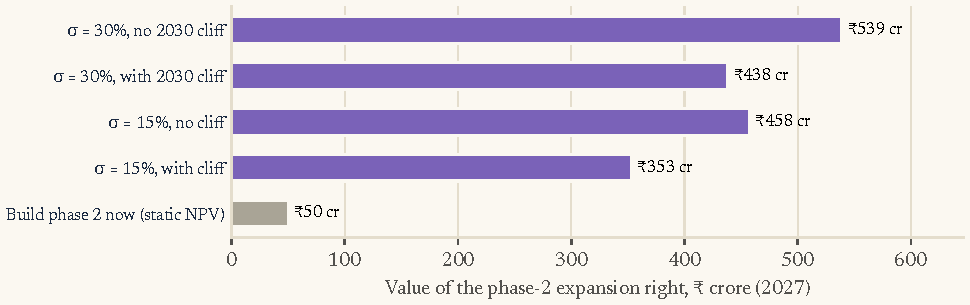
\includegraphics[width=\textwidth]{options.pdf}
\caption{Value of the right to build phase two, under two volatility assumptions, with and without the 2030 cliff. Source: \texttt{realoptions.expansion\_lsmc}.}
\end{figure}

\begin{center}\tablefont
\begin{tabularx}{\textwidth}{@{}L c c@{}}
\toprule
\thead{₹ crore, 2027 money} & \thead{Volatility 30\%} & \thead{Volatility 15\%}\\ \midrule
Build phase two now (static NPV) & 50 & 50\\
Option value with the 2030 cliff & 438 & 353\\
Option value without the cliff & 539 & 458\\
Cost of the cliff & 101 & 105\\
Never exercised (share of futures) & 43\% & 16\%\\
\bottomrule
\end{tabularx}
\end{center}

\begin{finding}[Three things the option model says that NPV cannot]
\textbf{First, wait.} Building phase two today is worth ₹50 crore; keeping the right to build it is worth ₹438 crore. The difference is the value of learning before committing. \textbf{Second, the cliff does not make us rush.} In most futures where phase two gets built, it is built late (2036), after the waiver has gone, because rushing in before costs fall is worse than losing the waiver. \textbf{Third, the cliff still has a price: about ₹100 crore.} That is the most we should ever pay to make an early phase two possible, for example by buying extra land, oversizing the grid connection, or pre-permitting a second train before 2028. \confL\ (for the levels), \confM\ (for the logic).
\end{finding}

\subsection{Option two: the AEM switch}
The 20 MW PEM slot will need new stacks around 2041. At that moment we can buy PEM again, or AEM if AEM has become cheap and, above all, durable. AEM promises PEM-like flexibility without iridium or platinum, but today's evidence on long-term durability is thin, and the leading listed AEM maker is still losing money \cite{enapter2026,enki2026}.

We model AEM's cost falling along Wright's law, a fixed percentage for every doubling of cumulative production \cite{wright1936}, with a learning rate between 8\% and 20\% and between three and eight doublings by 2041. Learning in energy models is itself uncertain and should be treated as such \cite{zeyen2023}. The chance that AEM proves durable (40,000+ hours) rises with deployment. ``Keeping the bay AEM-ready'' (compatible footprint, power electronics and water quality) costs \usd{}0.3--0.6 million now \estd.

\begin{center}\tablefont
\begin{tabularx}{\textwidth}{@{}L c@{}}
\toprule
\thead{Result} & \thead{Value}\\ \midrule
Expected value of the switch right (2030 money) & \usd{}1.46 million\\
Cost of keeping the bay ready & \usd{}0.3--0.6 million\\
AEM installed cost by the swap year, median & \usd{}777/kW\\
Chance we switch & 59\%\\
Chance AEM proves durable & 59\%\\
\bottomrule
\end{tabularx}
\end{center}

\begin{verdict}[Buy the option; let durability decide]
The option is worth roughly three to five times what it costs to keep, so we buy it. Notice that the chance of switching equals the chance AEM proves durable: in every future where AEM survives in the field, it is also cheaper by 2041. \textbf{The gate is not price; it is proof.} So the stage-gate for the switch is written in hours, not rupees: at least 40,000 hours of field data across several sites, an OEM warranty that covers degradation, and a pilot of 1--2 MW in our own bay before we commit the rest. \confM
\end{verdict}

\subsection{The stage-gates}
\begin{center}\tablefont
\begin{tabularx}{\textwidth}{@{}P{20mm} L L@{}}
\toprule
\thead{Gate} & \thead{Question} & \thead{Pass if}\\ \midrule
G0, 2027 & Start development? & Buyer term sheet signed; site AHP confirmed with real data.\\
G1, 2028 & Financial close? & Signed take-or-pay; EPC at or below \usd{}850/kW; P80 commissioning before 2031; base-case min DSCR $\geq$ 1.30.\\
G2, 2028 & Protect phase two? & Extra land and grid capacity cost less than \textasciitilde ₹100 crore.\\
G3, 2033+ & Build phase two? & Option model says exercise (value minus cost beats waiting); second buyer signed.\\
G4, 2039 & AEM in the bay? & 40,000 h field data; warranty; 1--2 MW pilot passes.\\
\bottomrule
\end{tabularx}
\end{center}
\newpage
